\subsection{Modelos del sistema.}\label{cap:modelos-sistema}

\subsubsection{Escenarios.}\label{cap:escenarios}
Para la siguiente sección se considerarán los actores Jugador 1 y Jugador 2, como Alice y Bob respectivamente.
\begin{itemize}
    \item \textbf{Jugador 1:} Usuario que juega el juego.
    \item \textbf{Jugador 2:} Usuario que juega el juego.
\end{itemize}

%Escenario
\begin{center}
    \begin{tabular}{ l | c  }
        Escenario:            & Alice y Bob recibe una mano \\
        Actores participantes: & Alice: Usuario  1                                              \\\hline
                                         & Bob: Usuario    2                                                 \\\hline
        Flujo de eventos:                & 1.-Los jugadores desean jugar cariocas                                      \\
                                         & 2.-Se barajan las cartas y luego se reparten 12 cartas\\\hline
                                         & aleatoriamente a cada jugador. \\\hline
        Condicion de Salida:             & 3.-Se muestra en pantalla el turno del jugador 1.                          \\\hline
        \hline
    \end{tabular}
    \\
    \begin{tabular}{ l | c  }
        Escenario:            & Alice retira una carta del mazo \\
        Actores participantes: & Alice: Usuario  1                                              \\\hline
        Flujo de eventos:                & 1.-Es el turno de Alice                                     \\
                                         & 2.-Alice retira una carta para iniciar su turno \\\hline
        Condicion de Salida:             & 3.-Se muestra en pantalla las cartas que Alice tiene en su mano \\\hline
         &incluyendo la carta nueva         \\\hline
        \hline
    \end{tabular}
    \\
    \begin{tabular}{ l | c  }
        Escenario:            & Alice retira una carta del mazo de descarte \\
        Actores participantes: & Alice: Usuario  1                                              \\\hline
        Flujo de eventos:                & 1.-Es el turno de Alice                                 \\
                                         & 2.-Alice ve una carta que le es de utilidad para su jugada. \\\hline
                                         & 3.-Alice retira una carta del mazo de descarte para iniciar su turno. \\\hline
        Condicion de Salida:             & 4.-Se muestra en pantalla las cartas que Alice tiene en su\\\hline
        &mano incluyendo la carta nueva                       \\\hline
        \hline
    \end{tabular}
    \\
    \begin{tabular}{ l | c  }
        Escenario:            & Alice logra juntar dos trios \\
        Actores participantes: & Alice: Usuario  1                                              \\\hline
        Flujo de eventos:                & 1.-Es el turno de Alice                                 \\
                                         & 2.-Alice roba una carta ya sea del mazo de descarte o el mazo tradicional.\\\hline
                                         & 3.-Alice se da cuenta de que hay juntado 2 trios y es lo que se pide en la ronda. \\\hline
                                         & 4.-Alice baja sus trios                      \\\hline
                                         & 4.-Finaliza su turno dejando una carta en el mazo             \\\hline
        Condicion de Salida:             & 5.-Se muestra en pantalla las cartas que alice bajó y las remanentes en su mano                   \\\hline
        \hline
    \end{tabular}
    \\
    \begin{tabular}{ l | c  }
        Escenario:            & Alice logra juntar una escala y un trio\\
        Actores participantes: & Alice: Usuario  1                                              \\\hline
        Flujo de eventos:                & 1.-Es el turno de Alice                                 \\
                                         & 2.-Alice roba una carta ya sea del mazo de descarte o el mazo tradicional.\\\hline
                                         & 3.-Alice se da cuenta de que hay juntado un trio y una escala, \\\hline
                                         &patron que se pide en la ronda. \\\hline
                                         & 4.-Alice baja su escala y trio                   \\\hline
                                         & 4.-Finaliza su turno dejando una carta en el mazo             \\\hline
        Condicion de Salida:             & 5.-Se muestra en pantalla las cartas que alice bajó y las remanentes en su mano                   \\\hline
        \hline
    \end{tabular}
    \\
    \begin{tabular}{ l | c  }
        Escenario:            & Alice bota una carta a Bob\\
        Actores participantes: & Alice: Usuario  1                                              \\\hline
                                         & Bob: Usuario  2                                              \\\hline
        Flujo de eventos:                & 1.-Es el turno de Alice                                 \\
                                         & 2.-Tiene en su mano una carta que coincide con el patrón de Bob.\\\hline
                                         & 3.-Decide botar la carta en el patrón de bob. \\\hline
                                         & 4.-Termina su turno descartando una carta               \\\hline
        Condicion de Salida:             & 5.-Se muestra en pantalla las cartas que alice botó\\\hline
                                            & y las remanentes en su mano. Además de las cartas que Bob tiene bajadas.             \\\hline
        \hline
    \end{tabular}
    \begin{tabular}{ l | c  }
        Escenario:            & Alice gana la ronda\\
        Actores participantes: & Alice: Usuario  1                                              \\\hline
                                         & Bob: Usuario  2                                              \\\hline
        Flujo de eventos:                & 1.-Es el turno de Alice                                 \\
                                         & 2.-Toma una carta del mazo.\\\hline
                                         & 3.-Decide botar la carta en el patrón de bob. \\\hline
                                         & 4.-Termina su turno descartando una carta               \\\hline
                                         & 5.-Alice gana la partida              \\\hline
        Condicion de Salida:             & 6.-Se muestra en pantalla la victoria de Alice.             \\\hline
        \hline
    \end{tabular}
    

\end{center}
\subsubsection{Modelos de casos de uso.}\label{cap:modelos-casos-uso}
\clearpage
\begin{figure}[h]
    \centering
    %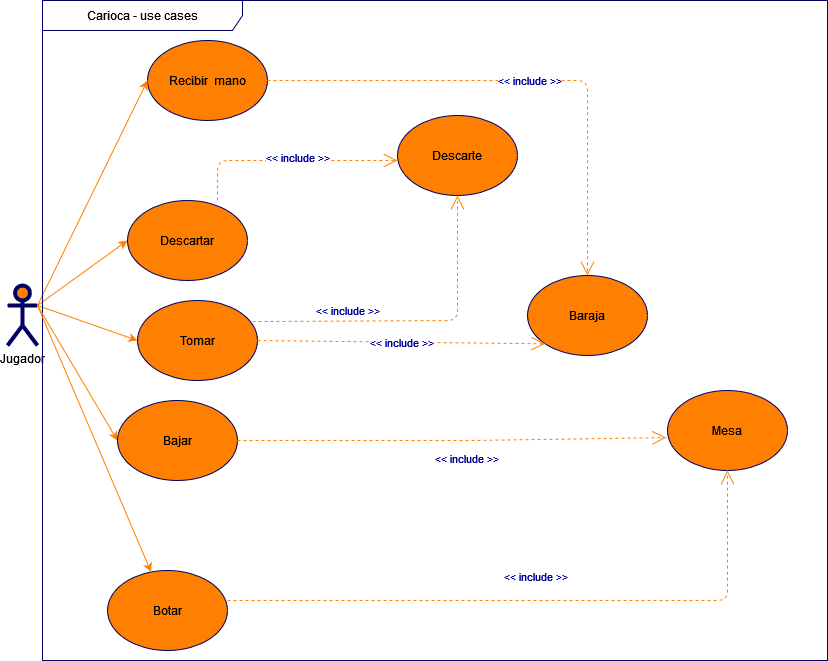
\includegraphics[width=15cm]{use-cases.png}
    \caption{Diagrama de casos de uso generalizado.}
\end{figure}
%CASO DE USO 1
\begin{center}
    \begin{tabular}{ l | c  }
        Nombre del caso de Uso: & Recibir mano                                    \\
        Actor participante:     & Iniciado por: Jugador                           \\\hline
        Condicion Inicial:      & 1. Debe ser la primera ronda                    \\
        Flujo de eventos:       & 2. El jugador recibe 12 cartas aleatoriamente   \\\hline
        Condicion de Salida:    & 3. Se muestra en pantalla el turno del jugador  \\
                                & 4. Se muestra en pantalla el Total de Cartas: N \\
                                & 5. Se muestra en pantalla Cartas en la mesa     \\
                                & 6. Se muestra en pantalla Cartas en descartes   \\
                                & 7. Se muestra en pantalla Cartas en la mano     \\
                                & 8. Se muestra en pantalla un menu de opciones   \\ 
    \end{tabular} \\
\end{center}
%FIN CASO DE USO 1
%CASO DE USO 2
\begin{center}
    \begin{tabular}{ l | c  }
        Nombre del caso de Uso: & Retirar carta de la baraja                      \\
        Actor participante:     & Iniciado por: Jugador                           \\\hline
        Condicion Inicial:      & 1. Debe ser el turno del jugador                \\
        Flujo de eventos:       & 2. El jugador retira una carta de la baraja     \\\hline
        Condicion de Salida:    & 3. Se muestra en pantalla la carta retirada     \\
                                & 4. Se muestra en pantalla el turno del jugador  \\
                                & 5. Se muestra en pantalla el Total de Cartas: N \\
                                & 6. Se muestra en pantalla Cartas en la mesa     \\
                                & 7. Se muestra en pantalla Cartas en descartes   \\
                                & 8. Se muestra en pantalla Cartas en la mano     \\
                                & 9. Se muestra en pantalla un menu de opciones   \\ 
    \end{tabular} \\
\end{center}
%FIN CASO DE USO 2
%CASO DE USO  3
\begin{center}
    \begin{tabular}{ l | c  }
        Nombre del caso de Uso: & Descartar carta de la mano                      \\
        Actor participante:     & Iniciado por: Jugador                           \\\hline
        Condicion Inicial:      & 1. Debe ser el turno del jugador                \\
        Flujo de eventos:       & 2. El jugador descarta una carta de su mano     \\\hline
        Condicion de Salida:    & 3. Se muestra en pantalla la carta descartada   \\
                                & 4. Se muestra en pantalla el turno del jugador  \\
                                & 5. Se muestra en pantalla el Total de Cartas: N \\
                                & 6. Se muestra en pantalla Cartas en la mesa     \\
                                & 7. Se muestra en pantalla Cartas en descartes   \\
                                & 8. Se muestra en pantalla Cartas en la mano     \\
                                & 9. Se muestra en pantalla un menu de opciones   \\ 
    \end{tabular} \\
\end{center}
%FIN CASO DE USO 3
%CASO DE USO 4
\begin{center}
    \begin{tabular}{ l | c  }
        Nombre del caso de Uso: & Bajar patrón                                    \\
        Actor participante:     & Iniciado por: Jugador                           \\\hline
        Condicion Inicial:      & 1. Debe ser el turno del jugador                \\
        Flujo de eventos:       & 2. El jugador baja un patrón                    \\\hline
        Condicion de Salida:    & 3. Se muestra en pantalla el patrón bajado      \\
                                & 4. Se muestra en pantalla el turno del jugador  \\
                                & 5. Se muestra en pantalla el Total de Cartas: N \\
                                & 6. Se muestra en pantalla Cartas en la mesa     \\
                                & 7. Se muestra en pantalla Cartas en descartes   \\
                                & 8. Se muestra en pantalla Cartas en la mano     \\
                                & 9. Se muestra en pantalla un menu de opciones   \\ 
    \end{tabular} \\
\end{center}
%FIN CASO DE USO 4
%CASO DE USO 5 Retirar carta del descarte
\begin{center}
    \begin{tabular}{ l | c  }
        Nombre del caso de Uso: & Retirar carta del descarte                      \\
        Actor participante:     & Iniciado por: Jugador                           \\\hline
        Condicion Inicial:      & 1. Debe ser el turno del jugador                \\
        Flujo de eventos:       & 2. El jugador retira una carta del descarte     \\\hline
        Condicion de Salida:    & 3. Se muestra en pantalla la carta retirada     \\
                                & 4. Se muestra en pantalla el turno del jugador  \\
                                & 5. Se muestra en pantalla el Total de Cartas: N \\
                                & 6. Se muestra en pantalla Cartas en la mesa     \\
                                & 7. Se muestra en pantalla Cartas en descartes   \\
                                & 8. Se muestra en pantalla Cartas en la mano     \\
                                & 9. Se muestra en pantalla un menu de opciones   \\ 
    \end{tabular} \\
\end{center}
%FIN CASO DE USO 5


\subsubsection{Diccionario de datos}\label{cap:diccionario-datos}
\begin{itemize}
    \item\textbf{Game}:Clase que se encarga de implementar las reglas y logica del juego, \\como tambien mostrar los datos necesarios por pantalla tal como el menu del sistema. 
    \item\textbf{Player}:Entidad que interactua con el juego, baraja y la baraja de descarte. Tiene la capacidad de tomar, dejar, botar cartas.
    \item\textbf{Card}:Clase para representar las cartas para el juego carioca, estas contienen un id, numero y pinta.
    \item\textbf{CardStack}:Clase Padre de Deck y DiscardDeck, la cual tiene como función almacenar instancias de la clase Card
    \item\textbf{Deck}:Clase hija de CardStack. Se almacenan instancias de la clase Cartas que son Generadas al principio del Juego
    \item\textbf{DiscardDeck}:Clase hija de CardStack. Se almacenan instancias de la clase Cartas que son descartadas por una instancia de la clase Player
    \item\textbf{Table}:Objeto de la clase Game, el cual almacena trios y escalas de los jugadores. 
\end{itemize}
\clearpage
\subsubsection{Diagrama de clases.}\label{cap:diagrama-clases}
A continuación se presenta el diagrama de clases del sistema a programar para el desarrollo del juego de cartas Cariocas:
\begin{figure}[H]
    \centering
    %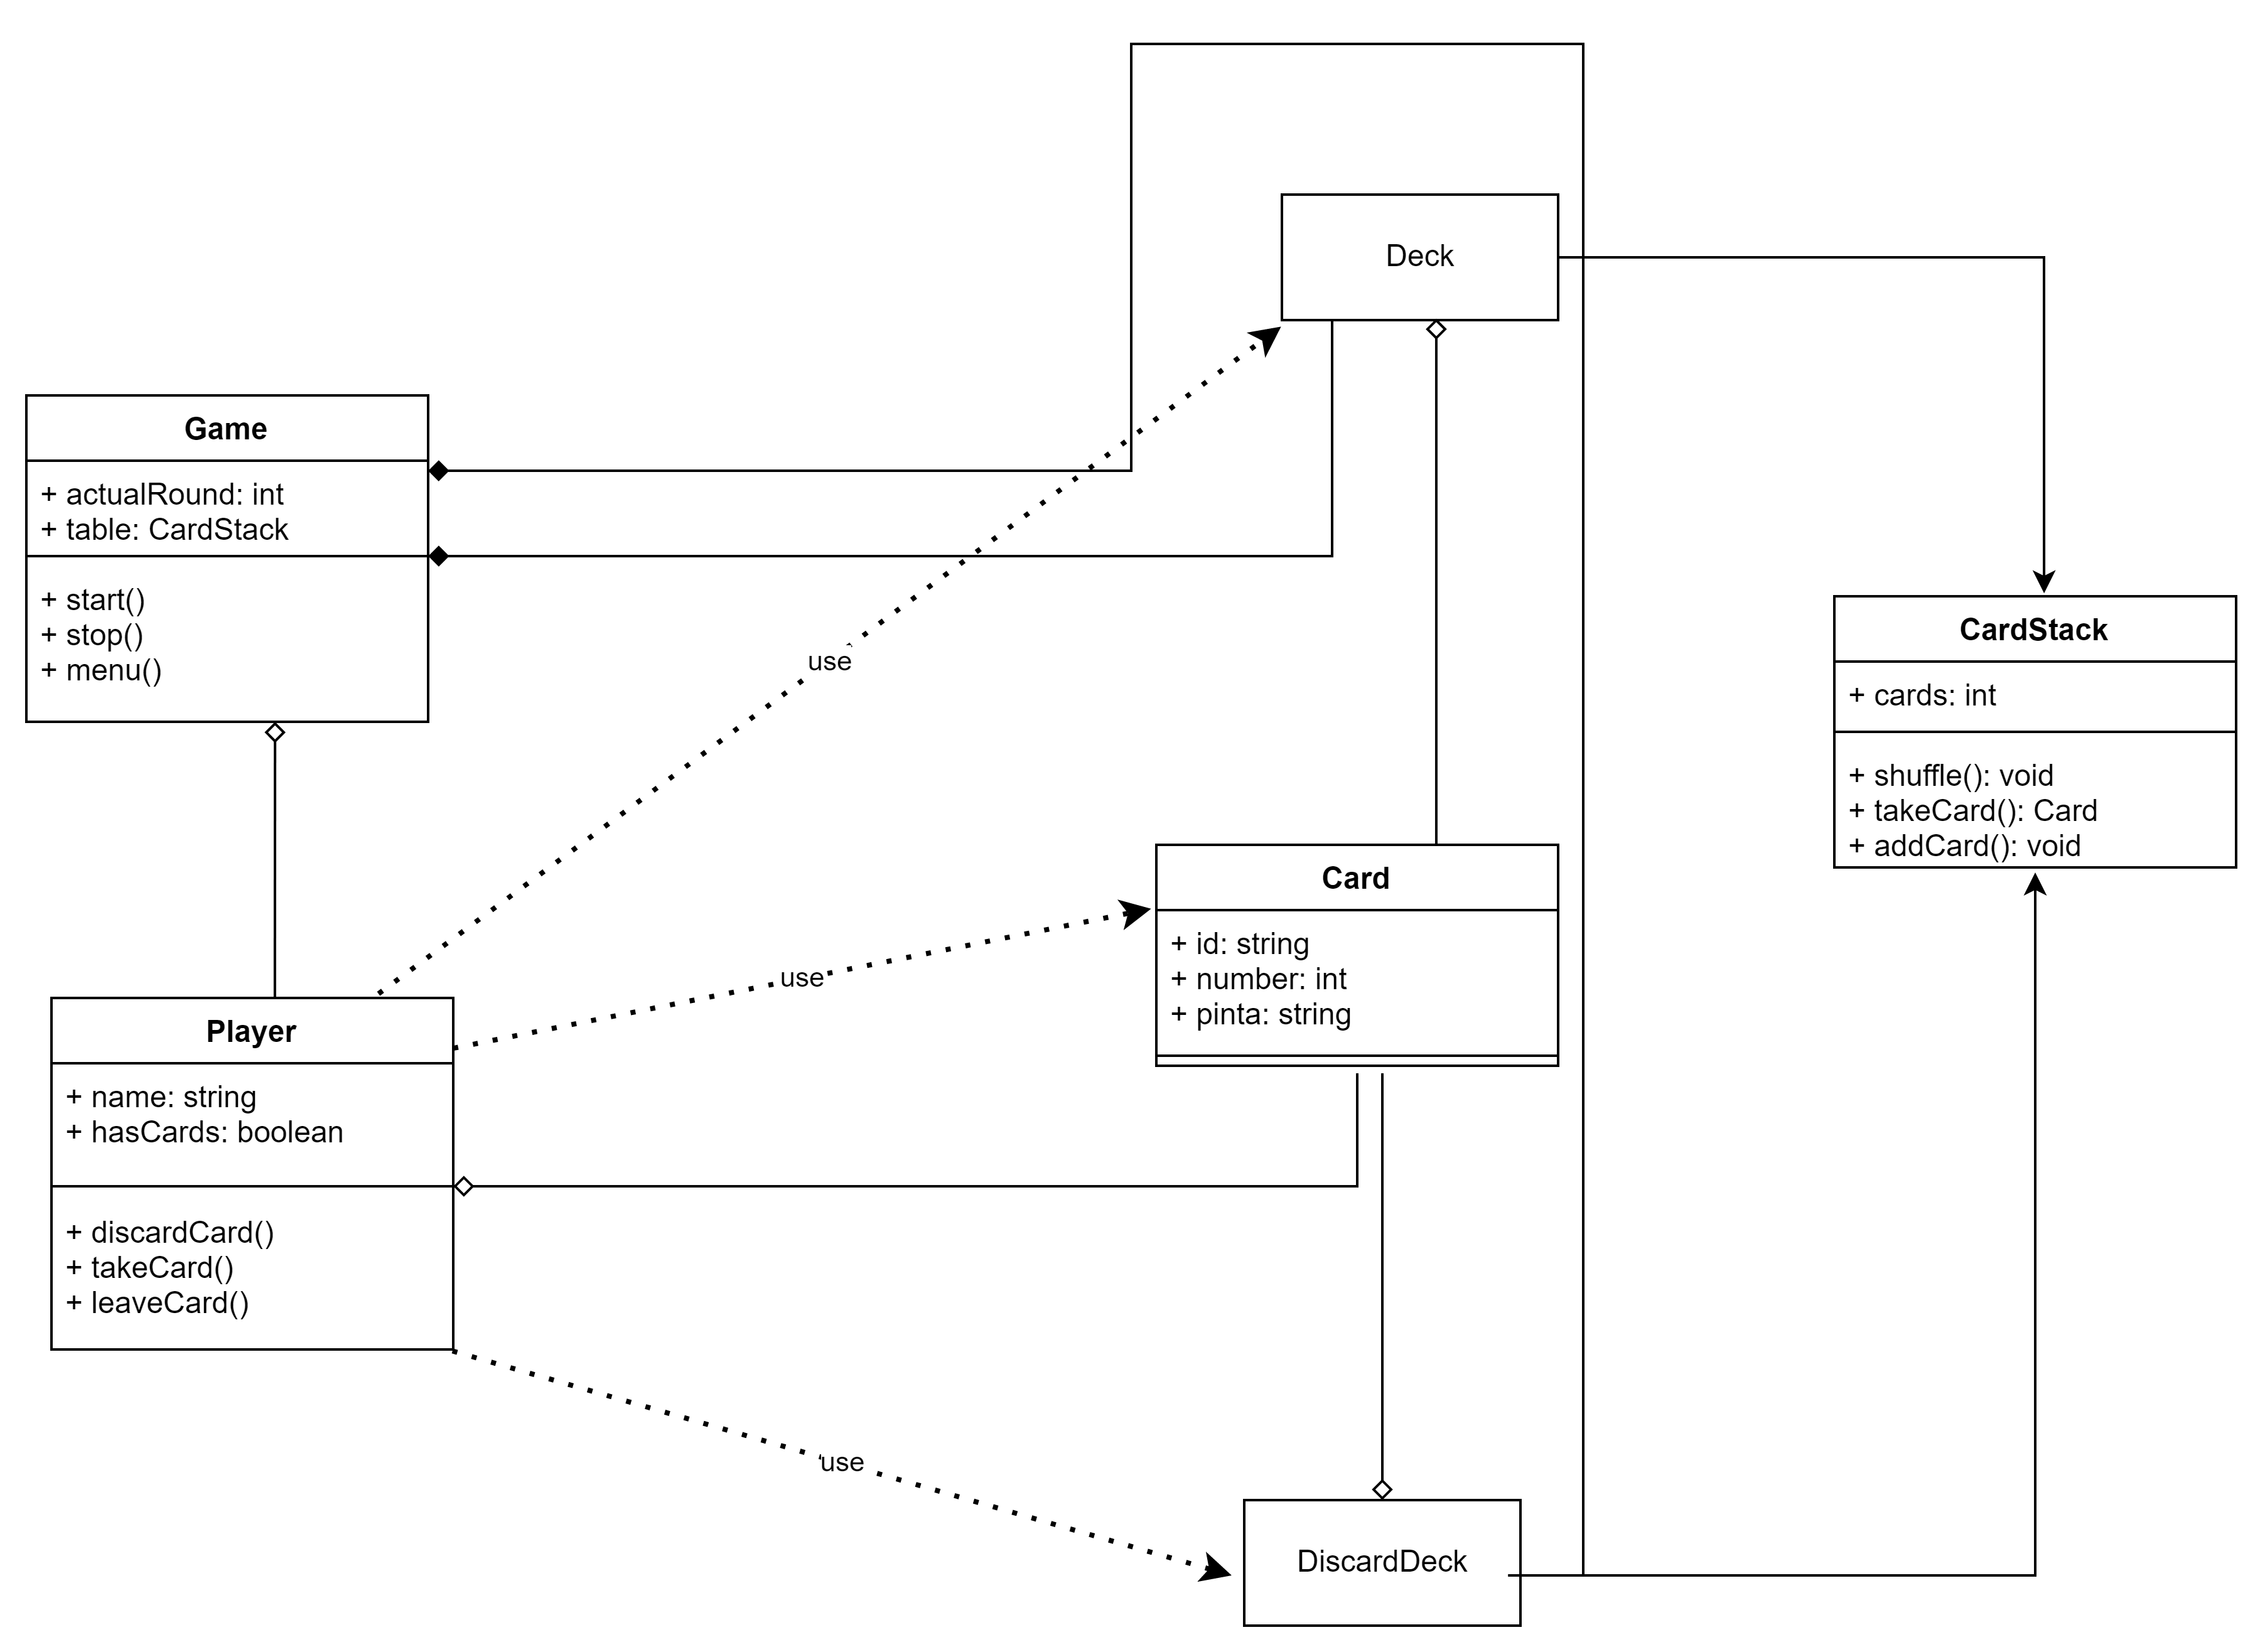
\includegraphics[width=15cm]{diclass.png}
    \caption{Diagrama de clases para el juego de cartas Cariocas.}
\end{figure}

\clearpage